% !TeX root = ../main.tex
% Add the above to each chapter to make compiling the PDF easier in some editors.

\chapter{Background}\label{chapter:background}

\section{Verifiable Credentials}

\acrfull{VC} is a recent \acrshort{W3C} standard for interoperable digital credentials on the Web that is cryptographically secure, tamper-evident, privacy respecting, and machine-verifiable" \parencite{Sporny.18Kas2019}. These credentials include but are not limited to passports, ID cards, university degrees, tickets etc. Any set of claims about a subject can be a credential. In the \acrshort{VC} setting these claims create \textit{subject-property-value} relationships that can be expressed in graphs. For instance being graduated from a university can be represented as the graph in Figure \ref{fig:alumniOf}. 

Subjects of claims are not necessarily persons and can be anything. In a peer review context a claim could be \textit{Peer Review-author-John Doe} where the subject is the peer review. Alternatively same relationship can be represented as \textit{John Doe-reviewerOf-Peer Review} where the subject is the person.

\begin{figure}[htbp]
  \centering
  \includesvg[width=0.8\textwidth]{claim-example}
  \caption{Example subject-property-value relationship of a graduation claim \parencite{Sporny.18Kas2019}} \label{fig:alumniOf}
\end{figure}

Although people usually associate credentials to be issued only by a respected authority such as a state, a university or a hospital, \acrlong{VC} allows anyone to issue claims. Yet, each credential is meaningful in a certain context and depending on the trust relationships between parties. An \textit{alumniOf} claim is only meaningful if issued by a university that is known to the employer in a job application or a \textit{goodHusband} claim only makes sense if issued by a spouse. Parties that receive a credential can choose to accept or reject a credential depending on the real world trust relationships.

A credential is a set of claims, i.e. a graph of information around a subject. Additional to the claims, the metadata and a digital proof form a verifiable credential. The proof is generally a digital signature of the claims and metadata, which makes the verifiable credential "verifiable".

\begin{figure}[htbp]
  \centering
  \includesvg[width=0.4\textwidth]{credential}
  \includesvg[width=0.8\textwidth]{credential-graph}
  \caption{Components of a verifiable credential and the graph of information of an example credential \parencite{Sporny.18Kas2019}} \label{fig:credentialGraph}
\end{figure}

The \acrshort{VC} specification models the stakeholders and interactions between them as in Figure \ref{fig:ecosystem}. \textit{Issuer}s assert claims and issue credentials about subjects, \textit{Verifier}s verify the credentials presented to them, and \textit{Holder}s aquire, store, and present credentials. Note that the subject of a credential can be different than its holder such as a pet being the subject and its owner being the holder, or a peer review as the subject and the reviewer as the holder. Finally, a \textit{Verifiable Data Registry} acts as the backend of these interactions by maintaining identifiers and schemas. This registry could be a distributed ledger or a central database depending on the implementation.

\begin{figure}[htbp]
  \centering
  \includesvg[width=0.8\textwidth]{ecosystem}
  \caption{Stakeholders of a \acrlong{VC} ecosystem and their roles \parencite{Sporny.18Kas2019}} \label{fig:ecosystem}
\end{figure}

\subsection{Verifiable Presentations}

The specification also describes an extension to the \acrshort{VC} data model that enables the packaging of multiple credentials and verification of the authorship of the data. A Verifiable Presentation consists of one or more verifiable credentials, presentation metadata, and a proof which is usually a digital signature of the first two. Credential holders can combine different credentials from different issuers for each use case, and the proof of the presentation provides the means to verify the authorship of data that the credentials are being presented by their intended holders and not someone else.

\begin{figure}[htbp]
  \centering
  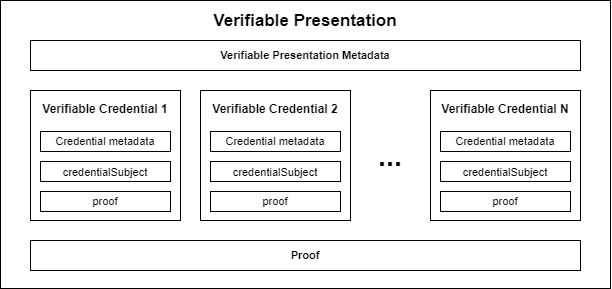
\includegraphics[width=0.8\textwidth]{figures/presentation.png}
  \caption{Outline of a verifiable presentation} \label{fig:presentation}
\end{figure}

\subsection{Syntax}

The data model provided in the \acrshort{VC} specification is an abstract representation of the information around a credential. For the exchange of the information a machine readable data exchange format or syntax is required. Popular data exchange formats are XML \parencite{xmlRFC}, \acrshort{JSON} \parencite{jsonRFC}, and \acrshort{YAML} \parencite{yaml}. Although any syntax can be used, the specification describes \acrfull{JSON-LD} \parencite{jsonld} and \acrshort{JSON} with \acrshort{JWT} \parencite{rfc7519} serializations of the data model. \acrshort{JSON-LD} is the preferred format for many applications including this work. A comparison of \acrshort{JSON-LD} over \acrshort{JWT} is available in the \acrshort{VC} implementation guide \parencite{chadwick_longley_sporny_terbu_zagidulin_zundel_2019} and is discussed in \cite{young_2021}. 

\acrshort{JSON-LD} is both an extension to \acrshort{JSON} and effectively a \acrfull{RDF}\footnote{https://www.w3.org/TR/rdf11-concepts/} syntax. The use of \acrshort{JSON-LD} accomplishes several things. First, it  brings linked data properties with minimal changes to \acrshort{JSON}, which is widely used in today's web. Second, it makes possible to model complex real world relationships with a graph model. Third, it enables "permissionless innovation" through extensibility. Anyone can extend the existing vocabularies and numerous cryptographic proof formats and signature suites can be used. This is in line with the "open world assumption" approach, that anyone can assert claims about any subject. It is up to implementers and verifiers to decide based on the real world trust relationships which claims to accept and which entities to trust. 

Originally, keys (attributes) in \acrshort{JSON-LD} documents are \acrfull{IRI}s \parencite{rfc3987}, which are similar to \acrfull{URI}s \parencite{rfc3986}
\footnote{The \acrshort{JSON-LD} spec uses \acrshort{IRI}s but the \acrshort{VC} spec only mentions \acrshort{URI}s so the two are used interchangeably. This document refers to identifiers as \acrshort{URI}s}. 
There's often confusion around \acrshort{URI}s, \acrshort{URL}s, and \acrshort{URN}s. Figure \ref{fig:uri} and the examples in Listing \ref{lst:uri} helps understanding the differences. Interested readers may refer to the relevant \acrshort{RFC} for further information \parencite{rfc3305}.

\begin{figure}[htbp]
  \centering
  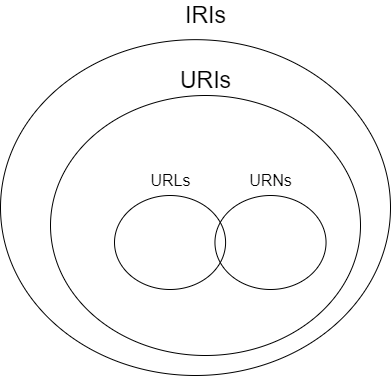
\includegraphics[width=0.5\textwidth]{URI.png}
  \caption{Identifiers}
  \label{fig:uri}
\end{figure}

\begin{lstlisting}[label={lst:uri}, caption={URL and URN examples}]
URL: ftp://ftp.is.co.za/rfc/rfc1808.txt
URL: http://www.ietf.org/rfc/rfc2396.txt
URL: telnet://192.0.2.16:80/
URL: did:ethr:0xb9c5714089478a327f09197987f16f9e5d936e8a
URN: isbn:0-486-27557-4
URN: uuid:6e8bc430-9c3a-11d9-9669-0800200c9a66
\end{lstlisting}


The use of identifiers lets machines to unambiguously refer things in the world. For instance the meaning of the property \lstinline{children} may be obvious for a human-reader depending on the context. If the reader sees the property under a person object, they can infer that it means "a son or a daughter of that person". However, \lstinline{children} is also used to express hierarchical relationships between things. These semantics need to be stated explicitly for machines to be able to "understand" what these properties stand for and to avoid such ambiguities in machine communication. That's why instead the keys are \acrlong{IRI}s. Also to avoid everyone defining their own \lstinline{child} semantics, shared vocabularies are defined. One popular vocabulary is \url{schema.org}. To express "a child of a person", the \acrshort{IRI} \url{https://schema.org/children} can be given. A \acrshort{JSON-LD} document expressing family relationships looks like in Listing \ref{lst:exampleJSONLD}

\begin{lstlisting}[language=json, label={lst:exampleJSONLD}, caption={A JSON-LD with full \acrshort{IRI}s}]
{
  "@id": "http://doefamily.net/john",
  "http://schema.org/givenName": "John",
  "http://schema.org/familyName": "Doe",
  "http://schema.org/children": {
    "@id": "http://doefamily.net/jane",
    "http://schema.org/givenName": "Jane",
    "http://schema.org/familyName": "Doe"
  }
}
\end{lstlisting}

However this document is difficult to read. Instead of having to write full \acrshort{IRI}s each time, a \lstinline{@context} can be included in the document that will map terms in the included document to \acrshort{IRI}s. Similar to a human communication, this sets the context of the information exchange, thus removing the ambiguity and providing conciseness. A context document for the previous \acrshort{JSON-LD} file might be as follows (Listing \ref{lst:exampleJSONLD-context}).

\begin{lstlisting}[language=json, label={lst:exampleJSONLD-context}, caption={A context file}]
{
  "@context": {
    "firstName": "http://schema.org/firstName",
    "lastName": "http://schema.org/lastName",
    "children": "http://schema.org/children"
}
\end{lstlisting}

Assuming the context is located at \lstinline{http://example.com/familyContext}, the previous document becomes more human-readable by embedding the context (Listing \ref{lst:exampleJSONLD-full}).

\begin{lstlisting}[language=json, label={lst:exampleJSONLD-full}, caption={A context added JSON-LD with shortened terms}]
{
    "@context": "http://example.com/familyContext",
    "@id": "http://doefamily.net/john",
    "givenName": "John",
    "familyName": "Doe",
    "children": {
        "@id": "http://doefamily.net/jane",
        "givenName": "Jane",
        "familyName": "Doe"
    }
}
\end{lstlisting}

The examples above are \acrshort{JSON-LD} documents but they are not verifiable credentials. For a document to be a valid verifiable credential they must have the following properties:
\begin{itemize}
    \item A \lstinline{@context} property with the first member \url{https://www.w3.org/2018/credentials/v1}.
    \item A \lstinline{type}\footnote{Alias to \lstinline{@type}, also \lstinline{@id} is aliased to \lstinline{id} in \acrshort{VC}} property that includes the type \lstinline{VerifiableCredential}.
    \item And the following properties: \lstinline{credentialSubject, issuer, issuanceDate, proof}
\end{itemize}

A minimal verifiable credential and a verifiable presentation in \acrshort{JSON-LD} format are shown in Listings \ref{lst:exampleVC} and \ref{lst:exampleVP}.

\lstinputlisting[language=json, caption={Example verifiable credential \parencite{Sporny.18Kas2019}},label={lst:exampleVC}]{code/exampleVerifiableCredential.json}

\lstinputlisting[language=json, caption={Example verifiable presentation \parencite{Sporny.18Kas2019}},label={lst:exampleVP}]{code/exampleVerifiablePresentation.json}

%%%%%%
%%%%%%  Public Key Crpyto and Zk proofs
%%%%%% 
\section{Public Key Crypto and JSON-LD}

\subsection{Digital Signatures}

At the heart of today's applications and protocols lies the public key cryptography. The encryption scheme is based on a pair of keys: a public key which can be shared publicly or with the verifying party, and a private key which must be kept absolutely secret except its owner. Hence, it is also called asymmetric cryptography. A user can encrypt a message with their private key, and publish the message and their public key. Anyone anyone can then decrypt the encrypted message with the public key which assures this message was encrypted by the owner of the corresponding private key. Also by encrypting messages with the public key, others can ensure only the owner of the corresponding private key can decrypt the message.

This encryption scheme can also be used to create digital signatures. Apart from the key generation there are two main methods in a digital signature scheme. The \textit{sign} function takes a message and a private key as inputs and generates a signature. The \textit{verify} function takes the message, the digital signature, and the public key as inputs and outputs a boolean value \lstinline{true} if the signature is valid or \lstinline{false} otherwise. Upon receiving a message and a signature, the receiver, if they know the public key of the sender, can verify it. By verifying the message the receiver can check two things:
\begin{enumerate}
    \item \textbf{Authenticity:} The message is indeed sent by the sender and not someone else
    \item \textbf{Integrity:} The message they receive is indeed the message sender sent and not tampered with
\end{enumerate}

Thanks to these properties digital signatures can be used to sign documents or software distributions. Public key cryptography and digital signatures create the backbone of the trust and security of today's web through \acrfull{TLS} \parencite{rfc8446} and X.509 digital certificates \parencite{rfc5280}.

There are different asymmetric key techniques, but most notable are the RSA \parencite{rivest1978method} and elliptic curve cryptography based systems such as \acrshort{ECDSA} \parencite{johnson2001elliptic} and \acrshort{EdDSA} \parencite{rfc8032}. Elliptic curve signature schemes may be based on different elliptic curves with different properties. For instance, Bitcoin uses the \acrshort{ECDSA} as the digital signature algorithm and Secp256k1 as its curve, which is the name of the curve used with specific parameters. Together, a signature algorithm and a curve will describe the communicating parties how to encrypt-decrypt or sign-verify messages.   

\subsection{Linked Data Proofs}

Digital signatures can be used to ensure the authenticity and the integrity of linked data, in particular of verifiable credentials. For a verifiable credential to be "verifiable", it has to contain a \lstinline{proof} property which is a digital signature over the contents of the credential. The data model is designed to be proof format agnostic but two implementations are widely used as proof formats and are explained in the specification. One of them is \acrshort{JWT}s which is also one of the syntaxes. The other one is the Linked Data Proofs \parencite{ldproofs} and used widely with the \acrshort{JSON-LD} syntax. 

A Linked Data Proof not only tells the verifiers how to verify a document, but also provides additional meta-data such as when the signature is created and what the purpose of the signature is. Again, the vocabulary is included in the document in a \lstinline{@context} entry and using this shared vocabulary i.e. a shared understanding of how to do a verification and what the signature stands for, the parties of a credential exchange can communicate unambiguously. With that, anyone can create a signature suite and a corresponding vocabulary that can be used in verifiable credentials. The original \acrshort{VC} context\footnote{https://www.w3.org/2018/credentials/v1} already contains some cryptographic suites. A security vocabulary is also available under W3C Credentials Community Group\footnote{https://w3c-ccg.github.io/security-vocab/}. Additional methods can be specified in the Linked Data Cryptographic Suite Registry\footnote{https://w3c-ccg.github.io/ld-cryptosuite-registry/}.

A Linked Data Proof has the following properties required \parencite{ldproofs}:

\begin{itemize}
    \item \textbf{type:} the name of the cryptographic suite used in the proof such as \lstinline{RsaSignature2018}, \lstinline{BbsBlsSignature2020}
    \item \textbf{proofPurpose:} expresses why a proof is created. Avoids the unintended use of the proof such as a verifiable credential proof (\lstinline{assertionMethod}) being used for authentication (\lstinline{authentication})
    \item \textbf{verificationMethod:} expresses how to verify the proof. Usually an identifier resolves to a document containing the keys used for the signature.
    \item \textbf{created:} when the proof is created
    \item \textbf{signature value:} a string representation of the signature created. The key can be \lstinline{jws}, \lstinline{proofValue} etc.
\end{itemize}

It may also contain other values such as a \lstinline{nonce} or a \lstinline{domain}.

Even though digital signatures ensure the integrity of credentials, they also prevent selective disclosure. A signature is only valid over the whole of the credential and therefore it is not possible to share only some parts of it verifiably. Selective disclosure is a desired property for the minimization of personal data, which is a common principle in privacy regulations such as \acrshort{GDPR} \parencite{gdpr, langheinrich_2001}.

There are several ways to achieve data minimization \parencite{Helmy.8May2020}. One way is to contact the issuer each time during the verification and request the required attributes securely. This, called \textit{just in time issuance}, is how information exchange is done through current federated identity providers such as a Google or Facebook log in. Another method is to introduce a trusted third party acting as a \textit{trusted witness}. Publons, in a way acts a trusted witness for the peer reviews and provides review data to parties when needed. Also, it is possible to achieve selective disclosure \textit{cryptographically}. 

Using cryptographical methods, there are also several ways selective disclosure may be achieved. An issuer can issue a separate credential for each of the attributes of the combined credential as \textit{atomic credentials}, which allows the holder to present the required attributes \parencite{Chadwick.2019}. It is also possible to use \textit{hashed values} in the credential. A holder may then provide the pre-images of the hashed values which they want to disclose to the verifier without having to share all the fields \parencite[961]{R.Mukta.2020}. Similarly, instead of storing the hash of the credential, a \textit{Merkle tree} of fields can be stored. A holder can present values of the desired attributes and the required hashes in the Merkle tree to enable verification of the disclosed attributes \parencite{Hitchens.9Eyl2018}. Finally, there exist digital signatures that support \textit{\acrfull{zk-proofs}} and the selective disclosure of the attributes such as Camenish-Lysyanskaya \parencite{camenisch2002signature}, and BBS+ signatures \parencite{boneh2004short, camenisch2016anonymous, lodder_looker_2020}.


\subsection{Zero-Knowledge Proofs}

Zero-knowledge proofs of knowledge are protocols in cryptography where a \textit{prover} can cryptographically prove to a \textit{verifier} the validity of a statement without sharing any other information than the fact that the statement is true. The field recently received more attention with the implementation of the privacy-preserving digital currency Zcash \parencite{E.BenSasson.2016}. Even though commonly referred as zero-knowledge proofs, it is useful to distinguish between \textit{proofs} and \textit{proofs of knowledge}. A proof is sufficient evidence for the truth of a proposition such as a proof for the statement that there exists a three coloring for a specific graph. A proof of knowledge is a proof for the knowledge of a piece of information such as a proof to the statement that one knows a three coloring for a specific graph \parencite{green_2017}. 

Properties of zero-knowledge proofs are as follows \parencite{Groth.2010}:
\begin{itemize}
  \item \textbf{Completeness:} If the statement is true, the verifier will be convinced by the proof the prover presents that the statement is true
  \item \textbf{Soundness:} If the statement is false, a malicious prover can not convince the verifier that it is true.
  \item \textbf{Zero-Knowledge:} If the statement is true, a malicious verifier does not learn anything else than the fact that the statement is true.
\end{itemize}

The first two properties are also requirements for interactive proofs. The work of \cite{Goldwasser.1985} has first introduced the third property of Zero-Knowledge. A proof in a zero-knowledge proof system is not deterministic but a probabilistic proof. Through many rounds it is possible to decrease the error to practically negligible values. \cite{Goldreich.1991} also show that with the assumption of an unbreakable encryption, it is possible to create a zero-knowledge proof for the graph coloring problem. This is significant since the graph coloring problem is NP-complete and every NP problem can be reduced to an NP-complete problem in polynomial time, meaning every problem in NP has a zero-knowledge proof. 

These initial zero-knowledge proofs are also interactive, that is the prover and the verifier need to exchange information on each round. Each time a proof needs to be made, the prover and the verifier need to be online and interact in multiple rounds, which makes the usability of the protocol difficult. Also, since the soundness of the proof relies on the randomness of the challenges of the verifier on each round, a third-party cannot be convinced by such a proof. By looking at the protocol transcript and the proof, they can not be assured if this randomness holds. \cite{Blum.1988} have shown that with a common reference string shared by the prover and the verifier, it is possible to create non-interactive zero-knowledge proofs. The common reference string need not be private, which makes non-interactive zero-knowledge proofs more practical than interactive ones.


\section{Decentralized Identifiers}

\acrfull{DID}s \parencite{reed_sporny_longley_allen_grant_sabadello_2021} are a new type of globally unique identifiers that do not depend on centralized identity providers or registries, and give their users full control of their identity. \acrshort{DID}s follow the \acrshort{URI} syntax with a \lstinline{did:} scheme followed by a method and the method specific identifier. Some examples of \acrshort{DID}s are given in Listing \ref{lst:did-example}.

\begin{lstlisting}[label={lst:did-example}, caption={\acrlong{DID} examples}]
did:example:123456789abcdefghi
did:example:123456789abcdefghi#key-1
did:example:123456789abcdefghi?versionTime=2021-05-10T17:00:00Z
// Ethereum 
did:ethr:0xb9c5714089478a327f09197987f16f9e5d936e8a
// Sovrin
did:sov:mnjkl98uipsndg2hdjdjuf7
// Public-key embedded DID
did:key:z6MkpTHR8VNsBxYAAWHut2Geadd9jSwuBV8xRoAnwWsdvktH
// Web
did:web:example.com
\end{lstlisting}

Each \acrshort{DID} resolves to a \acrshort{DID} document, similar to how \lstinline{http://www.example.com} resolves to an HTML file. Different methods have different resolvers and may have their own internal way of creating method specific identifiers. A \acrshort{DID} document describes the meta-data associated with the object it identifies in a \acrshort{JSON-LD} format. This may include the public keys associated, the controller of the document, the services and the service endpoints available for the described object etc. The \acrshort{DID} \lstinline{did:example:123456789abcdefghi} may resolve to the following document in Listing \ref{lst:did-doc-example} which describes two public keys assoicated with it for verification purposes, and one for authentication. It also expresses that this object is controlled by the \acrshort{DID} \lstinline{did:example:bcehfew7h32f32h7af3}, and a service associated with it. This may for instance be an identifier for an \acrshort{IoT} device with an \lstinline{EncryptedDataVault} owned by a user identified with \lstinline{did:example:bcehfew7h32f32h7af3}.

\begin{lstlisting}[language=json, label={lst:did-doc-example}, caption={Example \acrlong{DID} document \parencite{reed_sporny_longley_allen_grant_sabadello_2021}}]
{
  "@context": [
    "https://www.w3.org/ns/did/v1",
    "https://w3id.org/security/suites/ed25519-2020/v1"
  ]
  "id": "did:example:123456789abcdefghi",
  "controller": "did:example:bcehfew7h32f32h7af3",
  "verificationMethod": [{
      "id": "did:example:123456789abcdefghi#key-1",
      "type": "Ed25519VerificationKey2020", 
      "controller": "did:example:123456789abcdefghi",
      "publicKeyMultibase": "zH3C2AVvLMv6gmMNam3uVAjZpfkcJCwDwnZn6z3wXmqPV"
    }, 
    {
      "id": "did:example:123456789abcdefghi#key-2",
      "type": "Ed25519VerificationKey2020", 
      "controller": "did:example:123456789abcdefghi",
      "publicKeyMultibase": "Zpfs4h2fkcJCwDNam3uVAjZpwnZn6z3wXmo91LvLMv6A"
    }
  ],
  "authentication": [
    "#key-1"
  ],
  "service": [{
    "id": "did:example:123456789abcdefghi#vault",
    "type": "EncryptedDataVault",
    "serviceEndpoint": "https://edv.example.com/"
  }]
}
\end{lstlisting}

\acrshort{DID}s and \acrshort{VC}s are both part of the \acrfull{SSI} ecosystem. Still, both specifications are separate and do not depend on each other. Since \acrshort{DID}s are \acrshort{URI}s, they can be used in the fields that are required to be \acrshort{URI}s in verifiable credentials. This includes \lstinline{id} fields, \lstinline{issuer}, \lstinline{verificationMethod}. Using \acrshort{DID}s in \lstinline{issuer} and \lstinline{verificationMethod} leverages the public keys associated with \acrshort{DID}s and the verification can be done using the keys associated.
